\subsection{Les mappings, besoin de s'assurer que les données peuvent toutes
êtres portées par le modèles}

\textbf{Les Difficultés des Mappings entre Différents Modèles de Données : Dublin Core, RDF et LIDO }\newline

L’intégration de données hétérogènes dans des formats variés est un défi majeur dans la gestion des informations culturelles. Les institutions telles que les musées, les bibliothèques et les archives doivent souvent mapper ou convertir des données entre différents modèles de métadonnées.\newline

Le mapping, ou faire un mappage consiste à établir des correspondances entre différents modèles de données. On peut avoir besoin d’effectuer ce procédé lors d’une migration de données d’un système à un autre au sein d’une même institution. Dans notre cas, nous avons effectué cet exercice pour s’assurer que les données provenant des agrégateurs intermédiaires et des institutions partenaires du ministère, pouvaient bien être portées par le modèle LIDO. Pour faire cette vérification nous avons collecté et eu accès aux données telles qu’elles sont dans les bases de données des partenaires et nous les avons mappés pour voir comment elles pouvaient être intégrées dans le modèle LIDO. \newline

Comme nous l’avons expliqué précédemment, parmi les modèles utilisés par les partenaires, nous avons le  Dublin Core (DC), et les données exprimées en RDF (Resource Description Framework) ainsi que le format de l’export Joconde, et des formats propres à un agrégateur ou une institution.
Ces standards, présentent des divergences notables lorsqu'il s'agit de les aligner avec le LIDO. Les difficultés rencontrées lors du mappage entre ces modèles se situent à plusieurs niveaux : la sémantique, la granularité, la structure des données, et l'harmonisation des 
vocabulaires. Pour mieux comprendre ces défis, il est essentiel d’illustrer ces difficultés à travers des exemples concrets.
Les plus grandes difficultés que nous avons rencontré sont survenues ont été lors du mappage entre Dublin Core et LIDO, ou entre RDF et LIDO. Ces difficultés résident dans la disparité des concepts sémantiques. Chaque modèle a été conçu avec des objectifs spécifiques et des interprétations sémantiques propres. \newline

Prenons le concept de "contributeur". Dans Dublin Core, le terme "creator" fait référence à toute personne ou entité ayant participé à la création ou à l'élaboration d'une ressource. Cependant, cette définition est volontairement large pour s'adapter à différents types de ressources (livres, articles, pages web, etc.).\newline

Dans LIDO, le terme "créateur" est plus précisément subdivisé. Par exemple, un contributeur à une exposition d'art peut être catégorisé comme "peintre", "auteur", ou "photographe". Le modèle LIDO introduit une granularité plus fine avec des distinctions entre différents types de participants, chacun associé à un rôle précis dans la chaîne de production d’un objet culturel. En effet, le modèle Lido est composé d'éléments et d’attributs. Pour le créateur d’une peinture on modélise un événement de création de l'œuvre, dans lequel on intègre un élément “acteur” qui a pour attribut “créateur”, ou même “peintre” sur on veut être plus précis. 

\begin{figure}[h!]
	\centerline{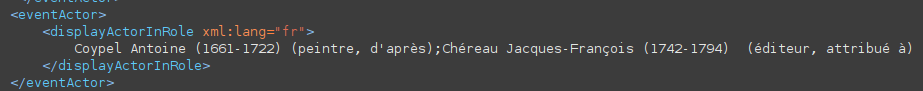
\includegraphics[width=\textwidth]{medias/figure_actor_2.png}}
	\caption{Exemple d'un peintre modélisé en LIDO}
\end{figure}
\begin{figure}[h!]
	\centerline{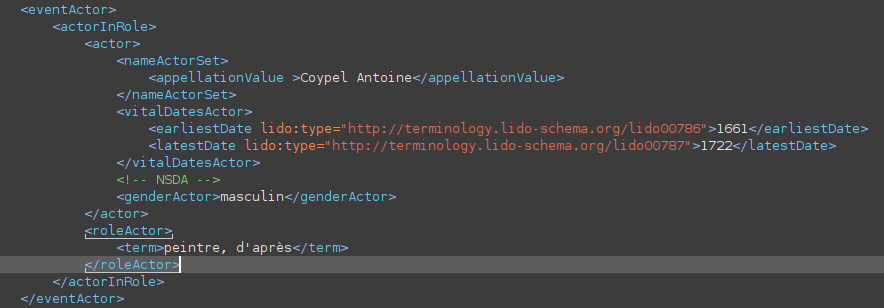
\includegraphics[width=\textwidth]{medias/figure_actor.png}}
	\caption{Exemple développé d'un peintre modélisé en LIDO}
\end{figure}

Lors du mappage, cette différence sémantique peut poser problème. Un contributeur générique dans Dublin Core doit être associé à un rôle spécifique dans LIDO. Si le rôle n'est pas précisé dans la source Dublin Core, il devient difficile de déterminer quelle sous-catégorie utiliser dans LIDO. Cette ambiguïté peut entraîner des erreurs de mappage ou la perte de détails importants.\newline

Dans le cas de RDF, les relations sont souvent exprimées de manière implicite à travers des triplets (sujet-prédicat-objet). Par exemple, une relation comme "Personne A a contribué à l'œuvre B" peut être définie de manière flexible, ce qui rend l’expression des rôles plus souple mais aussi moins spécifique. Pour adapter cette relation dans un cadre comme LIDO, il faudrait créer une correspondance précise, définissant le type de contribution en fonction des catégories disponibles dans LIDO.\newline

\textbf{Problèmes de Granularité}\newline

La granularité des données varie considérablement entre ces modèles, et cela devient particulièrement évident lors du mappage de données d'un modèle à un autre.\newline

Dans Dublin Core, l’élément "Date" est souvent utilisé pour désigner une date associée à la ressource. Cela peut inclure la date de création, la date de modification, ou la date de publication, mais le modèle ne fait pas de distinction claire entre ces différentes possibilités. Un document d'archive numérisé, par exemple, peut simplement avoir une seule date associée dans Dublin Core sans préciser s'il s'agit de la date de création ou d'une autre.\newline

En revanche, LIDO dispose de plusieurs éléments distincts pour capturer différentes dates liées à l’objet culturel, comme la "date de production", la "date d'acquisition", ou encore la "date d’exposition". Effet  cChaque date doit être associée à un événement, que ce soit un événement de création, d'acquisition, de découverte, etc…. Si on mappe des données de Dublin Core vers LIDO, la simple information de date ne suffit pas : il faut déterminer quelle catégorie de date correspond à celle fournie par Dublin Core, sinon on risque de perdre l’information..
Ce problème de granularité apparaît également lors du mappage de données RDF vers LIDO. Dans un graphe RDF, la date peut être liée à plusieurs entités ou événements par des relations spécifiques, mais ces relations ne correspondent pas toujours directement aux catégories de dates dans LIDO. Cela nécessite une analyse minutieuse du contexte RDF pour éviter une perte de précision lors du mappage. \newline

\textbf{Différences Structurelles}\newline

Les modèles de données Dublin Core, LIDO et RDF adoptent des structures très différentes, ce qui complique leur alignement.\newline

Dublin Core suit une structure relativement plate, avec des éléments de métadonnées tels que "titre", "créateur", "contributeur", et "sujet" placés au même niveau hiérarchique. Dans ce modèle, il n'y a pas de relation hiérarchique complexe entre ces éléments, et chaque élément se rapporte directement à la ressource décrite. Par exemple, une œuvre d’art dans Dublin Core pourrait être représentée avec un titre ("La Joconde"), un créateur ("Léonard de Vinci"), et une description simple.\newline

En revanche, LIDO utilise une structure hiérarchique plus complexe pour représenter les objets et leurs relations avec d'autres entités. Par exemple, une œuvre d’art serait décrite dans LIDO avec des sections distinctes pour le "titre", le "créateur", mais aussi pour des événements spécifiques comme l’acquisition, l’exposition, ou les restaurations. Ces événements sont eux-mêmes subdivisés avec des détails supplémentaires, tels que la date de l’événement, le lieu, et les participants. LIDO suit la structure en arborescence qui est commune aux modèles en XML.\newline

Le passage d’un modèle de structure plate (Dublin Core) à un modèle de structure structuré et hiérarchique (LIDO) nécessite souvent une réorganisation complète des données. Il faut non seulement redistribuer les éléments, mais aussi les relier de manière à respecter la hiérarchie de LIDO, sans pour autant perdre la qualité de la donnée. \newline

Dans RDF, les données sont souvent exprimées sous forme de graphes, où les relations sont définies comme des triplets entre des ressources. Si cette flexibilité est utile pour exprimer des relations complexes, elle nécessite une reformulation dans des systèmes comme LIDO, où les données doivent être présentées dans une structure hiérarchique. Par exemple, une relation RDF simple comme "Léonard de Vinci a peint la Joconde" peut devoir être traduite dans une structure LIDO où "Léonard de Vinci" serait placé dans une section distincte dédiée à l'événement de création de la Joconde, avec des métadonnées supplémentaires sur son rôle exact dans le processus créatif.\newline

Un autre défi crucial dans le processus de mappage est l'harmonisation des vocabulaires utilisés dans les différents modèles.\newline

Dans Dublin Core, les termes sont souvent choisis par l’utilisateur, avec peu d'obligation d'utiliser des vocabulaires contrôlés. Par exemple, pour l'élément "type", un utilisateur peut choisir d’indiquer simplement "peinture", tandis qu’un autre pourrait spécifier "huile sur toile". Ces deux entrées font référence à la même chose, mais ne sont pas normalisées.\newline

En revanche, LIDO dépend de vocabulaires contrôlés et de listes normatives pour assurer la cohérence et l'interopérabilité entre les institutions. Par exemple, une institution pourra choisir des termes précis provenant de thesaurus comme l’Art \& Architecture Thesaurus (AAT) pour décrire un objet et s'aligner sur ces thésaurus communs. \newline

Dans le cas de RDF, les vocabulaires peuvent également varier en fonction des données liées. Par exemple, une œuvre pourrait être associée à plusieurs schémas de classification RDF différents, chacun ayant sa propre ontologie. Lors du mappage vers LIDO, il faut non seulement traduire les termes RDF, mais aussi s'assurer qu'ils correspondent aux vocabulaires contrôlés utilisés dans le cadre LIDO, ce qui peut nécessiter l'utilisation d'outils de normalisation ou de ponts sémantiques. \newline
